\documentclass{article}

\usepackage{arxiv}

\usepackage[utf8]{inputenc} % allow utf-8 input
\usepackage[T1]{fontenc}    % use 8-bit T1 fonts
\usepackage{hyperref}       % hyperlinks
\usepackage{url}            % simple URL typesetting
\usepackage{booktabs}       % professional-quality tables
\usepackage{amsfonts}       % blackboard math symbols
\usepackage{nicefrac}       % compact symbols for 1/2, etc.
\usepackage{microtype}      % microtypography
\usepackage{subfigure}
\usepackage{float} 
\usepackage{graphicx}
\usepackage{caption}
\usepackage{lipsum}
\usepackage[utf8]{inputenc}
 
\usepackage{listings}
\usepackage{xcolor}
 
\definecolor{codegreen}{rgb}{0,0.6,0}
\definecolor{codegray}{rgb}{0.5,0.5,0.5}
\definecolor{codepurple}{rgb}{0.58,0,0.82}
\definecolor{backcolour}{rgb}{0.95,0.95,0.92}
 
\lstdefinestyle{mystyle}{
    backgroundcolor=\color{backcolour},   
    commentstyle=\color{codegreen},
    keywordstyle=\color{magenta},
    numberstyle=\tiny\color{codegray},
    stringstyle=\color{codepurple},
    basicstyle=\ttfamily\footnotesize,
    breakatwhitespace=false,         
    breaklines=true,                 
    captionpos=b,                    
    keepspaces=true,                 
    numbers=left,                    
    numbersep=5pt,                  
    showspaces=false,                
    showstringspaces=false,
    showtabs=false,                  
    tabsize=2
}
 
\lstset{style=mystyle}

\title{ECE269 Project Report}


\author{
  Jiaming Lai\\
  % \thanks{Use footnote for providing further
  %   information about author (webpage, alternative
  %   address)---\emph{not} for acknowledging funding agencies.} \\
  Department of Electrical and Computer Engineering\\
  University of California San Diego\\
  La Jolla, CA 92037 \\
  \texttt{jil136@ucsd.edu} \\
  %% examples of more authors
  %% \AND
  %% Coauthor \\
  %% Affiliation \\
  %% Address \\
  %% \texttt{email} \\
  %% \And
  %% Coauthor \\
  %% Affiliation \\
  %% Address \\
  %% \texttt{email} \\
  %% \And
  %% Coauthor \\
  %% Affiliation \\
  %% Address \\
  %% \texttt{email} \\
}

\begin{document}
\maketitle

% \begin{abstract}
%   We use 
% \end{abstract}
% % keywords can be removed
% \keywords{Eigenface \and Reconstruction}

\section{Introduction}
Following the "Eigenface" technique proposed by Matthew, et al.\ (1995)
\cite{eigenface1}\cite{eigenface2}, we derive eigenfaces (obtained via PCA) from face image
dataset. We use these eigenfaces (also known as principal components, PCs) to reconstruct different
kinds of images and evaluate the result via computing MSE. In section 2, we will cover a simplified
description of how the PCs are calculated and reconstruction is done. Combining with the singular 
values plot, we will give our justification of those PCs. Section 3-5 are about reconstruction result
using images from 190 individuals’ neutral expression image set, from 190 individuals’ smiling expression
image set and from the other 10 individuals’ neutral expression image set. In section 6, we will reconstruct
non-human images using all the PCs and evaluate the result. Section 7 is to reconstruct rotated images
and our comment of the result.

\section{Singular values plot and justification of PCs}
\subsection{Simplified description of PC computation and reconstruction}
As said in the Discussion 8, we construct covariance matrix $C$ from training image dataset:
\begin{equation}
  C = AA^T \nonumber
\end{equation}
In order to compute in an efficient way, we compute the eigenvector $v_i$ and its corresponding eigenvalues
$\mu_i$ of matrix $A^TA$. In our case, there should be 190 eigenvectors $v_i$ and eigenvalues $\mu_i$, because
we use first 190 individuals' neutral expression images to construct the covariance matrix $C$. We then translate
these 190 eigenvectors $v_i$ to eigenvectors for $C$:
\begin{equation}
  u_i = \frac{Av_i}{||Av_i||_2},\ where\ i=1,2,\ldots,190 \nonumber
\end{equation}
Given an image $\Gamma$, the reconstruction is as 
following:
\begin{equation}
  \hat{\Gamma} = \sum_{i=1}^{N}\omega_iu_i+\Psi \nonumber
\end{equation}
where $\omega_i=u_i^T(\Gamma-\Psi)$ and $N \le 190$ is number of PCs we want to choose. In section 2.3, we will
use the notation above to make more justification and explaination.

\subsection{Singular values plot}
Singular values $\sigma_i$ are obtained as following:
\begin{equation}
  \sigma_i = \sqrt{\mu_i},\ where\ i=1,2,\ldots,190 \nonumber
\end{equation}
Figure \ref{fig:fig1} is the singular values plot from data matrix.
\begin{figure}[h]
  \centering
  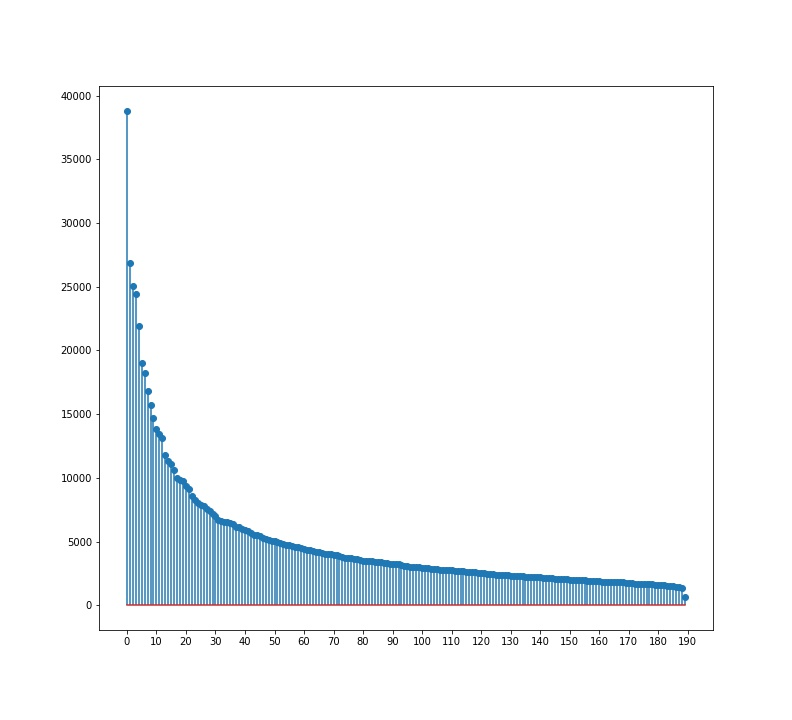
\includegraphics[width=0.8\textwidth]{../image/eigenvalues_neutral.jpg}
  \caption{Singular values plot}
  \label{fig:fig1}
\end{figure}

\subsection{Justification and explaination}
Suppose we want to choose $N$ PCs, which are also known as eigenfaces, then these PCs are actually eigenvectors
of $C$, $u_1,u_2,\ldots,u_N$, that corresponds to top eigenvalues $\mu_1,\mu_2,\ldots,\mu_N$. Suppose
$B=[u_1,u_2,\ldots,u_N]$, then because $u_i$ are orthogomal, matrix $BB^T$ is actually a projection matrix.
Given a image $\Gamma$, the reconstruction is actually project the raw image from $R(A)$ to $R(BB^T)$, while
$R(BB^T)$ is known as face space, having lower dimension than $R(A)$. When we compute MSE, we are actually computing
the norm distance between the raw image $\Gamma$ and the projected image $\hat{\Gamma}$. The number of PCs we choose
is depended on how large MSE we can stand. In pratice, there should be a threshod of MSE, we could always choose less
eigenvectors as PCs given the MSE is larger than the threshod.\\

The technique we use here is to reduce dimension. When we project the raw data onto a subspace (in our case, the subspace
is the face space), we could derive hyperplanes to classify different clusters. This technique is powerful not only because
it reduce the dimension and make computation efficiently, but also, by reducing dimension, we perform denoising on the data.

\section{Reconstruction result of problem (b)}

\subsection{MSE figures}
We randomly select three images from 190 individuals’ neutral expression image set and reconstruct each
of the images using using different number of PCs. We compute the mean squared error (MSE), see figure
\ref{fig:fig2}
\begin{figure}[h]
  \centering
  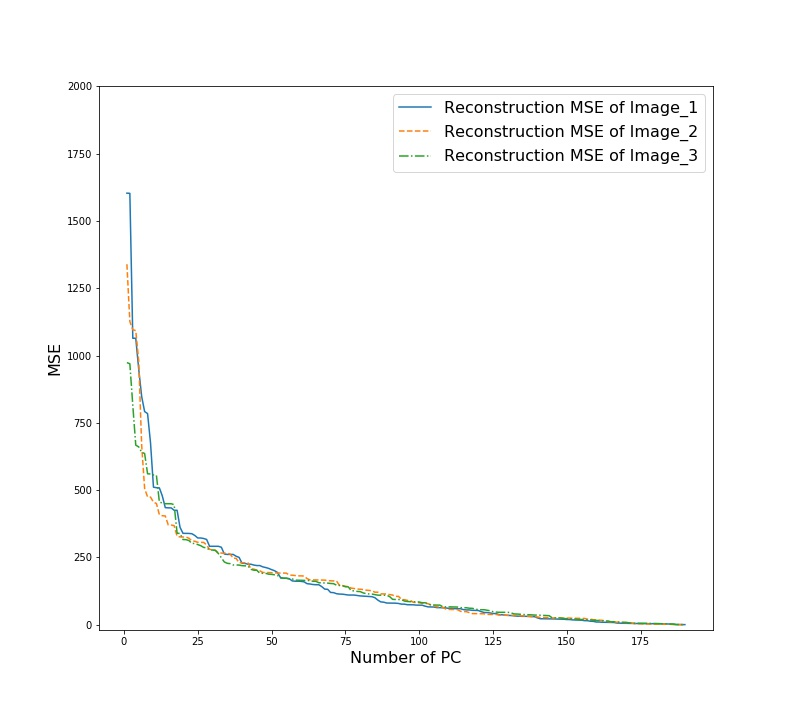
\includegraphics[width=0.8\textwidth]{../image/mse_neutral.jpg}
  \caption{MSE versus number of principal components\\ of 190 individuals’ neutral expression images}
  \label{fig:fig2}
\end{figure}

\subsection{Comment and explaination}
As we can see in figure \ref{fig:fig2}, when the number of PCs increases, the MSE of three randomly selected
images decrease and finally all converge to nearly zero. It is obvious because those PCs are derived from the
first 190 individuals’ neutral expression images. When we select one raw image from this 190 images set and use
more and more PCs to reconstruct it, the MSE would, off course, decrease to nearly zero.

\newpage
\section{Reconstruction result of problem (c)}

\subsection{MSE figures}
The same as section 3, we randomly select three images from 190 individuals’ smiling expression image set
and reconstruct each of the images using using different number of PCs. We compute the mean squared error (MSE), see figure
\ref{fig:fig3}
\begin{figure}[h]
  \centering
  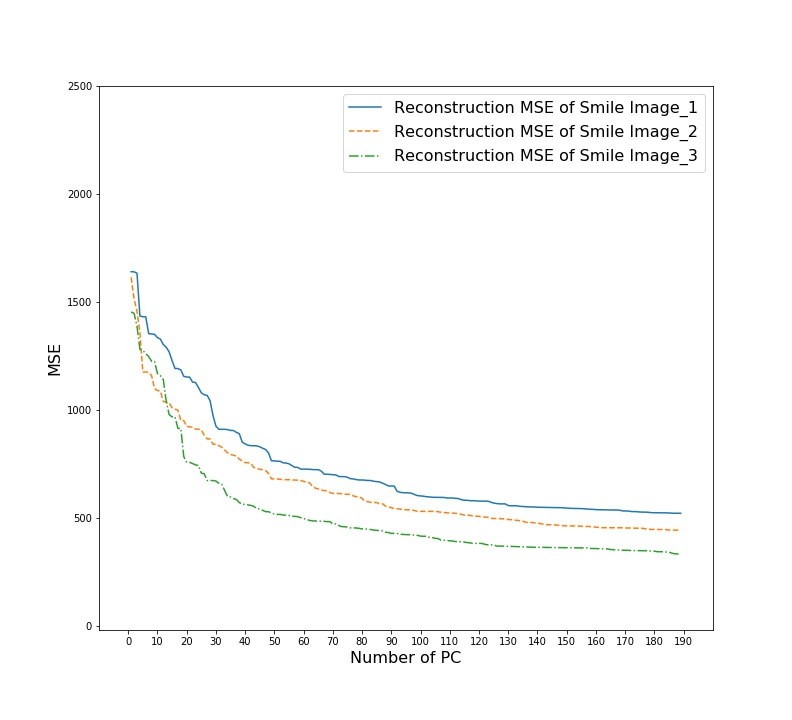
\includegraphics[width=0.8\textwidth]{../image/mse_smile.jpg}
  \caption{MSE versus number of principal components\\ of 190 individuals’ smiling expression image}
  \label{fig:fig3}
\end{figure}

\subsection{Comment and explaination}
The MSE of reconstruction of three randomly selected images have the same tendency. When the number of PCs
increases, the MSE decreases. But the MSE would not decrease to zero. When PCs' number is large enough, the
MSE converge to a bottleneck value. The bottlenelt value is about 500.\\

Because those three images are selected from 190 individuals’ smiling expression image set, so they are not
included in our training dataset. The PCs we obtained only capture the features related to our training data.
There are common features among smiling faces and neutral faces. This explains why the MSE would decrease. But
there should be some special features of smiling faces, which results in the bottleneck value of MSE.

\section{Reconstruction result of problem (d)}

\subsection{MSE figures}
The same as section 3-4, we randomly select three images from the other 10 individuals’ neutral expression image set
and reconstruct each of the images using using different number of PCs. We compute the mean squared error (MSE), see figure
\ref{fig:fig4}
\begin{figure}[h]
  \centering
  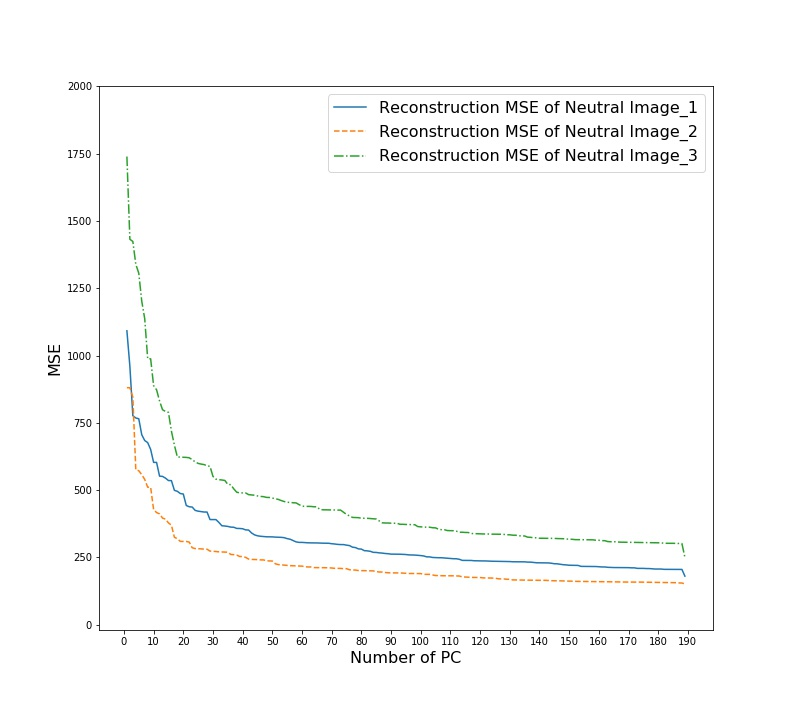
\includegraphics[width=0.8\textwidth]{../image/mse_other_neutral.jpg}
  \caption{MSE versus number of principal components\\ of the other 10 individuals’ neutral expression image}
  \label{fig:fig4}
\end{figure}

\subsection{Comment and explaination}
The same as the MSE line of figure \ref{fig:fig4}, 1.when the number of PCs increases, the MSE decreases. 2.When
the number of PCs is large enough, the MSE would reach its bottleneck value. The bottleneck value is about 250.
3.As we can see, the bottleneck value is obviously lower than the bottleneck value of figure \ref{fig:fig3}.\\

Because we are using neutral expression images for reconstruction in this section and those images are not included
in the training dataset, so when reconstruction, the projected face would be outside the boundary of cluster of
projected faces of training dataset. This results in the the bottleneck value. However, the projected face is
nearer to the cluster, comparing with the projected face of smiling image. This is why the the bottleneck value
of this section is lower than the bottleneck value of figure \ref{fig:fig3}.

\section{Reconstruction result of non-human image}

\subsection{Reconstruction result}
We use an apple image to perform reconstruction. The reconstruction result is shown in figure \ref{fig:subfigureExample}.
\begin{figure}[ht]
  \centering
  \subfigure[Original image]{
    
\includegraphics[width=0.3\textwidth]{../image/apple_crop.jpg}
    \label{fig:subfig1}
    }
    \subfigure[Reconstruction using all PCs]{
      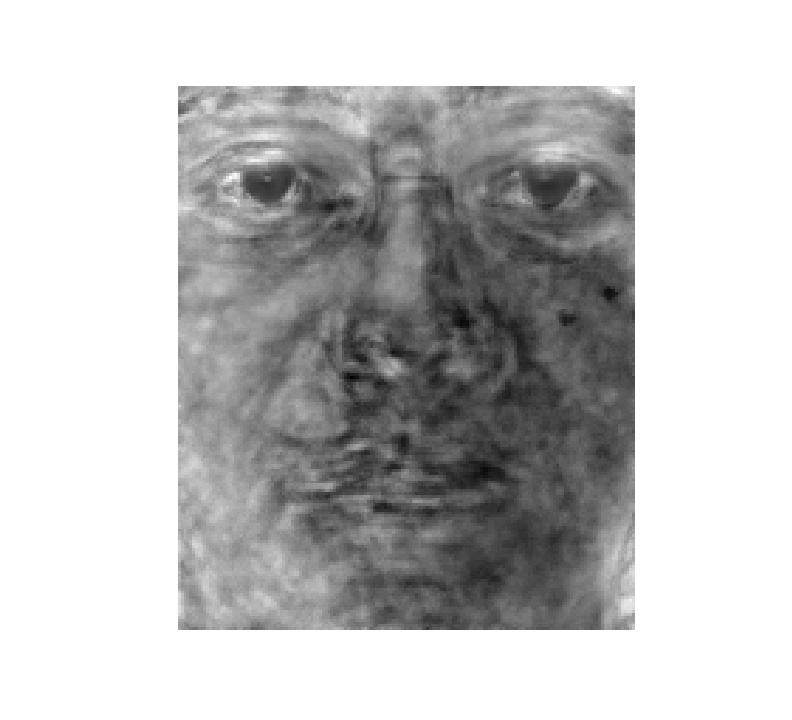
\includegraphics[width=0.3\textwidth]{../image/apple_reconstruct.jpg}
      \label{fig:subfig2}
    }
    \subfigure[Reconstruction plot in 'jet' mode]{
      
\includegraphics[width=0.3\textwidth]{../image/apple_reconstruct_jet.jpg}
      \label{fig:subfig3}
    }
    \caption[Reconstruction result of apple image]{Reconstruction result of apple image using all PCs}
    \label{fig:subfigureExample}
  \end{figure}

\subsection{Comment and explaination}
Figure \ref{fig:subfig2} display in 'gray' colormap and Figure \ref{fig:subfig3} display in 'jet' colormap.
We are using all PCs generated from neutral expression image data. So when reconstruction, it will force the
result to be like a face, just as we can see in figure \ref{fig:subfig2}. However, if we take a look at figure
\ref{fig:subfig3}, the blue area corresponds to the 'apple' area in original image. The yellow and red area corresponds
to the background in original image. So the reconstruction actually save much information of the original image,
especially those edges. This means that the PCs we generated use much feature from edges and fringes.

\section{Reconstruction result of rotated image}

\subsection{Reconstruction result}
In this section, we randomly select one face image from 190 individuals’ neutral expression images, rotate it
with different degrees, from -90 to 90. And then, we reconstruct the rotated images using all PCs.
Figure \ref{fig:rotatedimage} shows some examples of rotated images, as well as the original image.
\begin{figure}[ht]
  \centering
  \subfigure[Rotate with -45 degree]{
    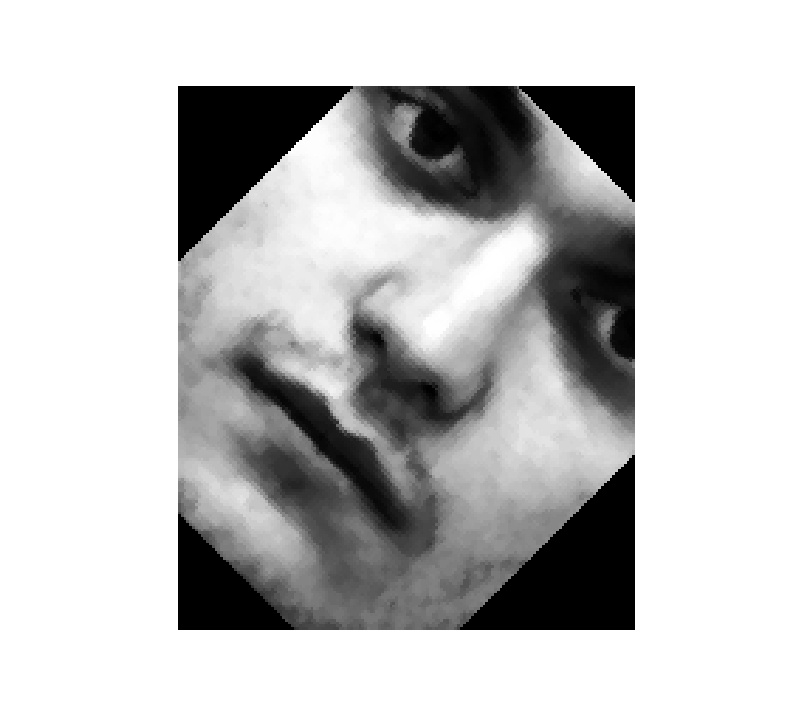
\includegraphics[width=0.3\textwidth]{../image/select_image_rotate-45.jpg}
    \label{fig:subfig4}
    }
    \subfigure[Original image]{
      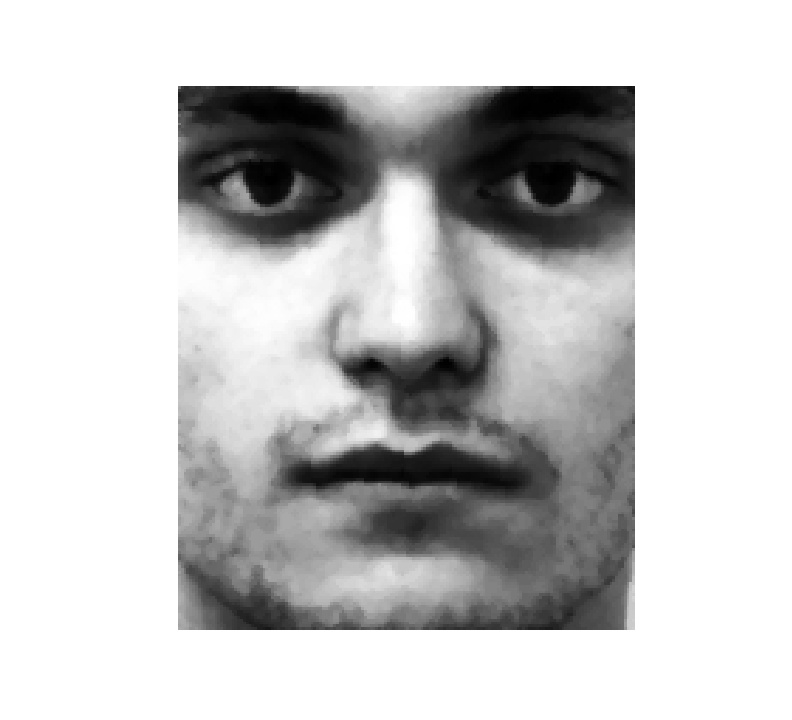
\includegraphics[width=0.3\textwidth]{../image/select_image.jpg}
      \label{fig:subfig5}
    }
    \subfigure[Rotate with 45 degree]{
      
\includegraphics[width=0.3\textwidth]{../image/select_image_rotate45.jpg}
      \label{fig:subfig6}
    }
    \caption[Reconstruction result of apple image]{Selected image and rotated images}
    \label{fig:rotatedimage}
  \end{figure}
\begin{figure}[h]
  \centering
  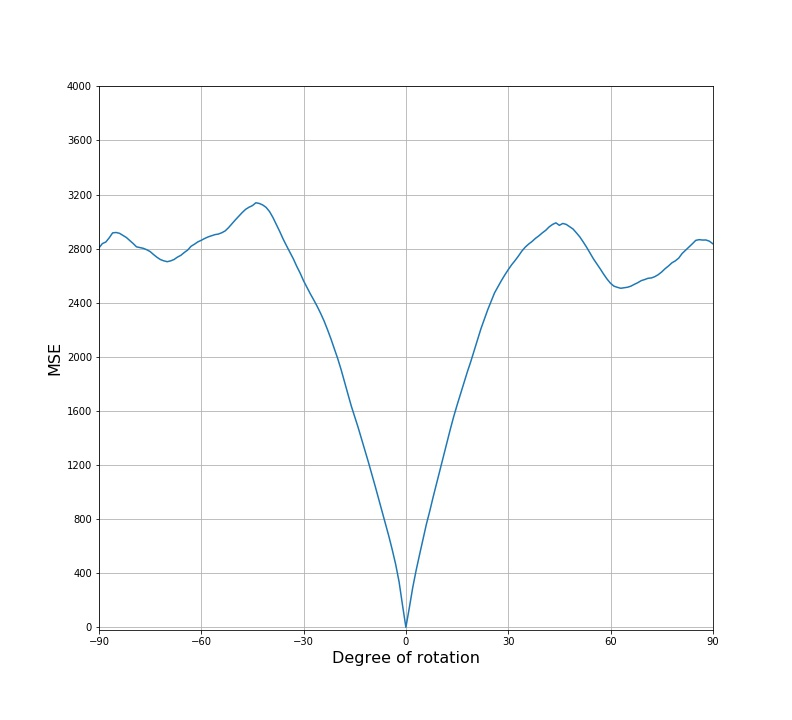
\includegraphics[width=0.8\textwidth]{../image/mse_rotate.jpg}
  \caption{MSE versus different rotate degrees}
  \label{fig:fig7}
\end{figure}
\\

\subsection{Comment and explaination}
As shown in figure \ref{fig:fig7}, when rotation degree increases, MSE would increase. When the degree reaches
about 40 or -40, MSE value steps into fluctuation. It is not surprising because the rotated image is actually a
new face image. In pratice, when we are doing face recognition, we should consider the effect of roration.
Because just as we see in figure \ref{fig:fig7}, even a small rotation degree would result in large MSE.

\bibliographystyle{unsrt}  
%\bibliography{references}  %%% Remove comment to use the external .bib file (using bibtex).
%%% and comment out the ``thebibliography'' section.
\bibliography{references}

\section*{Appendix}

The following is the Matlab code.

\subsection*{eigenface.py}
\lstset{style=mystyle}
\lstinputlisting[language=Python]{../eigenface.py}

\subsection*{data\_utils.py}
\lstset{style=mystyle}
\lstinputlisting[language=Python]{../data_utils.py}

\end{document}